\documentclass[12pt,a4paper]{article}
\usepackage[utf8]{inputenc}
\usepackage[T1]{fontenc}
\usepackage{listings}
\usepackage{color}
\usepackage{hyperref}
\usepackage{geometry}
\usepackage{graphicx}
\geometry{left=2cm,right=2cm,top=2cm,bottom=2cm}
\usepackage{needspace}

\title{SEARCH1DO: Search-Based Planning in Advanced 3D Environments}
\author{Oltion Nezha}
\date{24 Gennaio, 2025}

\begin{document}

\maketitle
\tableofcontents
\bigskip

\section{Introduzione e Obiettivi}
\Needspace{5\baselineskip} 
\subsection*{Obiettivi del Progetto}
\begin{itemize}
    \item Sviluppare un ambiente simulato per la risoluzione di labirinti.
    \item Implementare diversi algoritmi di ricerca (A*, Dijkstra, Uniform Cost).
    \item Analizzare e confrontare le performance degli algoritmi.
\end{itemize}

\Needspace{10\baselineskip}
\section{Descrizione del Progetto}
\textbf{SEARCH1DO Search-Based Planning in Advanced 3D Environments}

Questo progetto è stato realizzato per il corso \textit{Introduzione all'Intelligenza Artificiale} dell'Università degli Studi di Milano-Bicocca. L'obiettivo principale è sviluppare e testare algoritmi di pianificazione basata sulla ricerca in ambienti 3D complessi, sfruttando librerie avanzate per la simulazione 3D e la fisica (ad es. NVIDIA Cosmos, NVIDIA Omniverse, Project Chrono, PyBullet).

\medskip
\textbf{Integrazione con Gymnasium:}
\begin{itemize}
    \item Implementazione di algoritmi di ricerca fondamentali (ad es. A*, Uniform Cost, etc.).
    \item Valutazione delle performance in ambienti 3D semplici.
    \item Stima del costo computazionale in base alle caratteristiche dell'ambiente.
\end{itemize}

\section{Struttura del Progetto}
\Needspace{8\baselineskip}
\subsection*{Organizzazione delle Cartelle e File Principali}
\begin{samepage} 
\begin{verbatim}
Gymnasium/
  ├─ config.py              % Configurazioni ambiente, controller, etc.
  ├─ main.py                % Script principale per esecuzione simulazione
  ├─ README.md              % Documentazione base
  ├─ requirements.txt       % Dipendenze
  ├─ algorithms/
  │   ├─ astar.py           % Algoritmo A*
  │   ├─ dijkstra.py        % Algoritmo Dijkstra
  │   └─ uniform_cost.py    % Algoritmo Uniform Cost Search
  ├─ controllers/
  │   └─ pd_controller.py   % Controllore PD per il percorso
  ├─ envs/
  │   └─ maze.py            % Ambiente labirinto
  └─ utils/
      └─ conversion.py      % Conversione coordinate
\end{verbatim}
\end{samepage}

\section{Differenze tra Algoritmi di Ricerca}
\Needspace{6\baselineskip}
\textbf{A* vs Dijkstra vs Uniform Cost Search:}
\begin{itemize}
    \item \textbf{A*}: Combina il costo accumulato con una funzione euristica che stima il costo residuo fino al goal, migliorando l'efficienza della ricerca.
    \item \textbf{Dijkstra}: Espande i nodi basandosi esclusivamente sul costo accumulato, senza euristica. Garantisce il percorso più breve, ma può risultare meno efficiente.
    \item \textbf{Uniform Cost Search}: Simile a Dijkstra, espande i nodi in ordine crescente di costo accumulato. In questo progetto, è particolarmente utile per gestire terreni differenti, poiché consente di assegnare costi specifici (ad es. acqua, sabbia, strada) in base alla difficoltà di attraversamento.
\end{itemize}

\Needspace{8\baselineskip}
\section{Maze e Ambiente di Simulazione}

\begin{figure}[htbp]
    \centering
    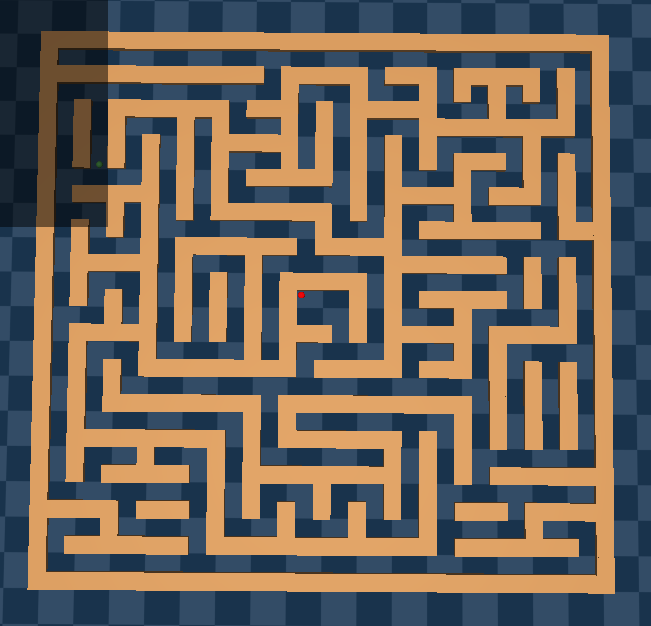
\includegraphics[width=0.7\textwidth]{image.png}
    \caption{Labirinto utilizzato nella simulazione.}
    \label{fig:maze}
\end{figure}

Il labirinto viene creato tramite una funzione che sfrutta \texttt{Gymnasium} per registrare e istanziare l'ambiente. Nel file \texttt{maze.py} vengono definiti due tipi di labirinti:
\begin{itemize}
    \item \textbf{LARGE\_MAZE}: un labirinto standard.
    \item \textbf{LARGE\_MAZE\_CUSTOM\_TERRAIN}: un labirinto con terreni personalizzati, dove vengono specificati costi differenti per tipi di terreno (ad es. acqua, sabbia, strada). Quest'ultimo viene utilizzato dall'algoritmo Uniform Cost per gestire il costo variabile di attraversamento.
\end{itemize}

La funzione \texttt{get\_maze(custom\_terrain)} permette di scegliere quale labirinto utilizzare, mentre \texttt{get\_maze\_dimensions(maze)} restituisce il numero di righe e colonne. Inoltre, i parametri per il rendering (come larghezza, altezza e seed) e per la configurazione dell'ambiente sono definiti all'interno del file.

\Needspace{40\baselineskip}
\section{Processo di Esecuzione}

\subsection*{Come Eseguire il Progetto}
\begin{itemize}
    \item Installare le dipendenze:
\begin{lstlisting}[language=bash]
pip install -r requirements.txt
\end{lstlisting}
    \item Avviare la simulazione specificando l'algoritmo:
\begin{lstlisting}[language=bash]
python Gymnasium/main.py --algorithm astar
\end{lstlisting}
\end{itemize}

\Needspace{6\baselineskip}
\subsection*{Dettagli del Processo di Simulazione}
\begin{itemize}
    \item \textbf{Ricerca del percorso}: Dopo aver calcolato i percorsi in modalità discreta, il percorso viene ottimizzato per velocizzare la simulazione.
    \item \textbf{Conversione in coordinate continue}: Il percorso ottimizzato viene trasformato per guidare l'agente nell'ambiente.
    \item \textbf{Controllo proporzionale-derivativo}: Il PD Controller gestisce la navigazione lungo i waypoint estratti dal percorso.
\end{itemize}

\section{Visualizzazione e Performance}
\Needspace{6\baselineskip}
\subsection*{Metriche e Visualizzazione}
\begin{itemize}
    \item Viene riportato il tempo di esecuzione e il numero di nodi espansi per ogni algoritmo.
    \item La simulazione mostra il percorso realizzato nel labirinto attraverso la funzione di rendering di Gymnasium.
\end{itemize}

\Needspace{30\baselineskip}
\section{Considerazioni Finali e Prospettive Future}
\begin{itemize}
    \item Implementazione di ulteriori algoritmi di ricerca per confronti più estesi.
    \item Gestione avanzata degli errori e introduzione di ulteriori metriche di performance.
    \item Possibile integrazione con altri ambienti di simulazione 3D (PyBullet, Nvidia Omniverse e Cosmos).
\end{itemize}

\section{Conclusioni}
\Needspace{6\baselineskip}
Il progetto SEARCH1DO rappresenta una solida base per la sperimentazione e lo sviluppo di algoritmi di pianificazione in ambienti 3D complessi. L'integrazione con librerie avanzate e l'uso di terreni personalizzati, in particolare per gestire costi variabili nell'algoritmo Uniform Cost, offrono spunti interessanti per ulteriori ricerche e miglioramenti futuri.

\end{document}
